\documentclass[11pt]{article}
\setlength{\arrayrulewidth}{0.5mm}
\setlength{\tabcolsep}{18pt}
\renewcommand{\arraystretch}{1.5}
\usepackage{tabularx}
\usepackage{adjustbox}
\usepackage{multirow}
\usepackage{tocloft}
\usepackage{tikz}
\usepackage[sorting=none]{biblatex}
\addbibresource{ref.bib}
\renewcommand\cftsecfont{\Large\bfseries}
\renewcommand\cftsecpagefont{\Large\bfseries}
\renewcommand\cftsubsecfont{\large\bfseries}
\renewcommand\cftsubsecpagefont{\Large\bfseries}
\usepackage[table,xcdraw]{xcolor}
% \usepackage[showframe]{geometry}
\usepackage{layout}
\usepackage{booktabs}
\usepackage{varwidth}
\usepackage[left=.5in, right=.5in, bottom=.5in, top=.5in]{geometry}
\usepackage{ragged2e}
\usepackage{graphicx} % Required for inserting images
\usepackage{listings}
\usepackage{float}
\usepackage{verbatim}
\usepackage{color}
\definecolor{dkgreen}{rgb}{0,0.6,0}
\definecolor{gray}{rgb}{0.5,0.5,0.5}
\definecolor{mauve}{rgb}{0.58,0,0.82}

\lstset{frame=tb,
  language=Python,
  aboveskip=3mm,
  belowskip=3mm,
  showstringspaces=false,
  columns=flexible,
  basicstyle={\small\ttfamily},
  numbers=none,
  numberstyle=\tiny\color{gray},
  keywordstyle=\color{blue},
  commentstyle=\color{dkgreen},
  stringstyle=\color{mauve},
  breaklines=true,
  breakatwhitespace=true,
  tabsize=3
}
\graphicspath{{./logo/}}
\setlength{\voffset}{-.75in}
\setlength{\textheight}{650pt}
% \setlength{\textwidth}{470pt}
% \setlength{\oddsidemargin}{0pt}
\setlength{\topmargin}{0pt}
% \setlength{\marginparsep}{0pt}
% \setlength{\hoffset}{0in}
\setlength{\marginparwidth}{1in}
\setlength{\headsep}{5pt}
\title{\huge \textbf{EmoSight: AI-Enabled Facial Emotion Visualization}\vspace{-2em}}
\date{\LARGE July 2023}











\begin{document} %\layout
\maketitle
{\centering{\huge{\textbf{CS F407: Artificial Intelligence}}}\par}
\vspace{0.25in}
\thispagestyle{empty}
\begin{center}
    
\includegraphics[scale=1]{logo/bits-logo.pdf}\\
\end{center}
\vspace{0.25in}
{\centering \LARGE{Under the supervision of\\ \textbf{Dr. Aneesh Chivukula}}\par}
\vspace{.75in}
{\centering
\begin{table}[b]
    {\centering \LARGE
    \begin{tabular}{|c|c|} \hline \centering
        \textbf{Group Members} & \textbf{ID}\\\hline
        Arya V Singalwar& 2020B3A71861H \\\hline
        M Varun Srinivas  & 2020B3AA0497H\\
        \hline \centering
        P Sai Shruthi & 2020B3A70904H\\
        \hline
    \end{tabular}\par}
\end{table}\par}
\pagebreak

\begin{center}
    \section*{\LARGE Abstract}
\end{center}
\thispagestyle{empty}
The rapid advancements in facial expression recognition research offer profound implications for businesses and psychological research. This study presents a comprehensive exploration of a facial emotion recognition model developed using Convolutional Neural Networks (CNN) for seven distinct emotions: anger, contempt, disgust, fear, happiness, sadness, and surprise. This emotion recognition is pivotal for tailoring businesses' strategies to customer emotions and identifying potential areas of improvement in products or services. The model can also monitor employee emotions for efficiency and effectiveness. The dataset comprised 981 images and was preprocessed and resized using Google Colaboratory. Data augmentation techniques, such as horizontal flipping and random shifts, were applied to enhance the dataset. The developed CNN model, consisting of several layers including convolutional, max-pooling, dropout, and dense layers, achieved an accuracy rate of 78.17\%, surpassing the pre-set threshold of 75\%. This model has wide-ranging applications from marketing to psychology, assisting in understanding cross-cultural emotions and aiding individuals who find it challenging to express their feelings. The model, deployed on a website using the Streamlit library, offers inputs through image uploads, widening its reach and usability. This facial emotion recognition model can significantly contribute to various domains by offering actionable insights into human emotions.

\pagebreak
\Huge{\textbf{Contents}}
\vspace{.1in}
    \hrule height 0.25mm
\vspace{0.15in}
\tableofcontents
\thispagestyle{empty}
\pagebreak
\clearpage
\pagenumbering{arabic}
\section{Introduction}
\normalsize{In recent years, research and development in the field of facial expression recognition have become more and more popular. There are many uses for effectively classifying a person's emotional state based on their facial expressions in many professions. Accurately classifying emotions, in particular, can be a helpful skill in business.

The problem describes that to offer the most excellent service, businesses must comprehend a customer's emotional state. An angry or disappointed consumer, for example, could require a different strategy than a happy or satisfied one. Businesses can deliver customised services and raise customer satisfaction by identifying a consumer's emotional state.

Businesses may better understand their clients by using facial emotion recognition. Businesses might spot areas for product or service improvement by analysing trends in consumer emotions. For instance, if a lot of customers complain, there may be an issue with that product or service that has to be fixed.

Emotion detection can also keep track of workers' emotions to ensure they carry out their tasks effectively and efficiently. An employee may need extra help or training if they exhibit signs of stress or dissatisfaction, for instance.

The seven categories of emotion—anger, contempt, fear, surprise, happiness, sadness, and disgust—can help us grasp people's feelings more subtly. Business needs this categorisation since it enables a more accurate depiction of a customer's emotional condition. Additionally, it can assist organisations in identifying different emotions that are more frequently linked to particular goods or services, enabling them to adjust their strategy accordingly.

In conclusion, there are many business applications for facial emotion recognition and classification. Businesses can offer personalised services, raise customer happiness, and spot improvement opportunities by precisely comprehending and categorising a customer's emotional state. A more sophisticated knowledge of a person's emotional state is provided by classifying seven different emotions, which can assist firms in adapting their strategy.
From this, we arrive at the following business objectives:
\begin{itemize}
    \item \textbf{Legal Proceedings} - Facial emotion detection helps us provide outputs on an individual’s emotional state by analysing facial expressions. It helps provide non-verbal cues that can help convey valuable information about a person’s attitude and demeanor. It helps remove bias and preconceived notions in humans while judging a person. \cite{legal}
    \item \textbf{Psychological Research} - Facial Emotion detection can help in therapy sessions, where some individuals cannot articulate their feelings entirely to their therapist. It can also help in the cross-cultural comparison of emotion.
\end{itemize}
}
\section{Data Preprocessing}
\normalsize{For the purpose of this project, the data has been sourced from a Kaggle dataset \cite{kaggle} with 7 emotions: Anger, Contempt, Disgust, Fear, Happy, Sadness, and Surprise.}
\subsection{Data Understanding}
\normalsize{The dataset contains a total of 981 images. The distribution of the images is as follows:
\begin{enumerate}
    \item Anger - 135
    \item Contempt - 54
    \item Disgust - 177
    \item Fear - 75
    \item Happy - 207
    \item Sadness - 84
    \item Surprise - 249
\end{enumerate}
The dataset does not show a high imbalance; hence, oversampling was not done for rebalancing the dataset. All the images in the dataset were in .png format, and OpenCV was used to work with these images.}
\subsection{Data Preparation}
The downloaded data was in .zip format. The preparation of the data to be used for training and testing purposes was done directly using \textit{Google Colaboratory} due to higher computing power availability. The input images were of size 244x244, and to use them with our model, they were resized to 48x48.
\begin{center}
    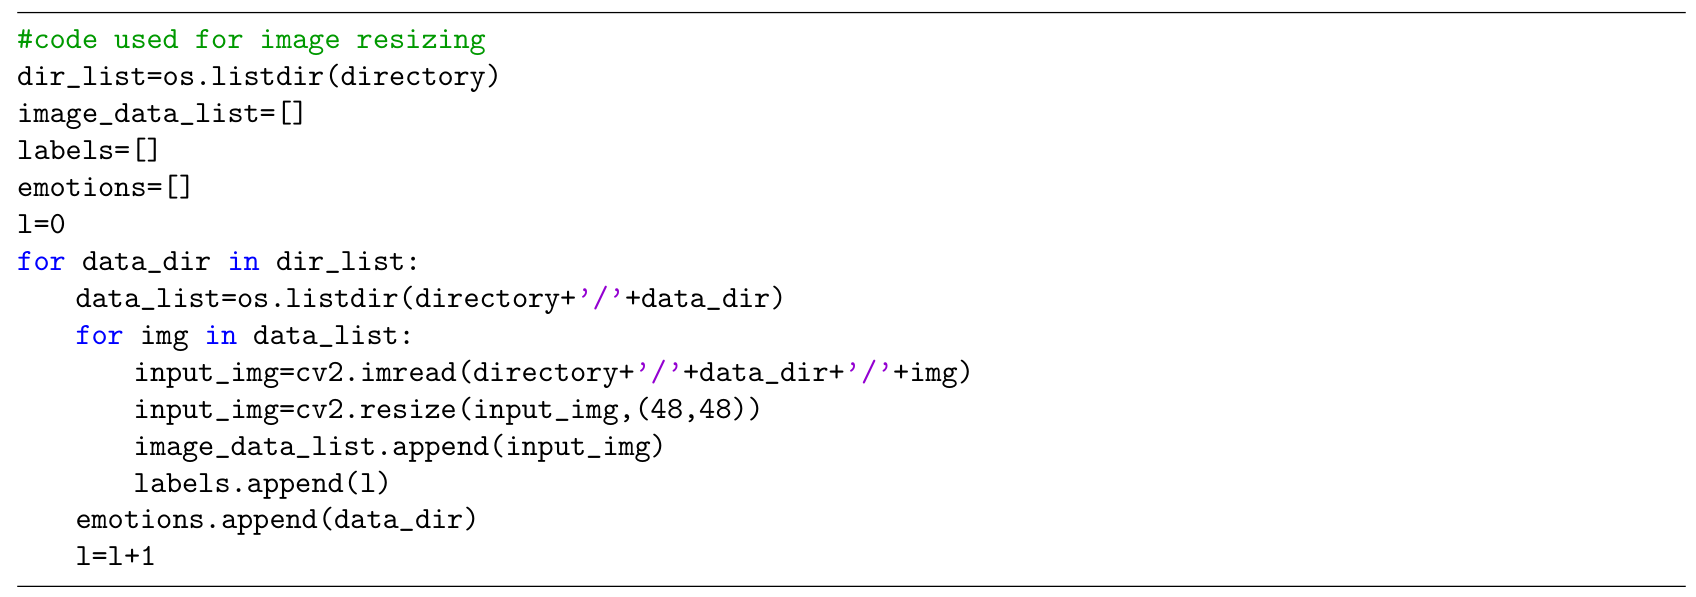
\includegraphics[scale=0.55]{code/fcode1.png}
\end{center}
% \begin{lstlisting}
% #code used for image resizing
% dir_list=os.listdir(directory)
% image_data_list=[]
% labels=[]
% emotions=[]
% l=0
% for data_dir in dir_list:
%     data_list=os.listdir(directory+'/'+data_dir)
%     for img in data_list:
%         input_img=cv2.imread(directory+'/'+data_dir+'/'+img)
%         input_img=cv2.resize(input_img,(48,48))
%         image_data_list.append(input_img)
%         labels.append(l)
%     emotions.append(data_dir)
%     l=l+1
% \end{lstlisting}
\section{Model Development}
The necessary libraries such as NumPy, Pandas, and OpenCV \cite{opencv} for data manipulation and image processing were imported. The code was run to iterate through the dataset and resize the images to store them in a NumPy array.
\begin{center}
    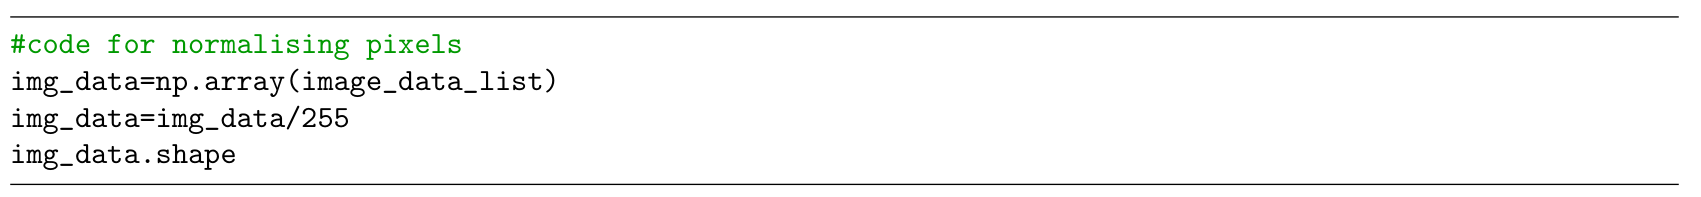
\includegraphics[scale=0.55]{code/fcode2.png}
\end{center}
% \begin{lstlisting}
% #code for normalising pixels
% img_data=np.array(image_data_list)
% img_data=img_data/255
% img_data.shape
% \end{lstlisting}
The images were then normalized by dividing their pixel values by 255 since the value for a pixel can range from 0 to 255. After this, the dataset was split into test and training data using the scikit-learn library. \cite{scikitlearn}
\pagebreak
\begin{center}
    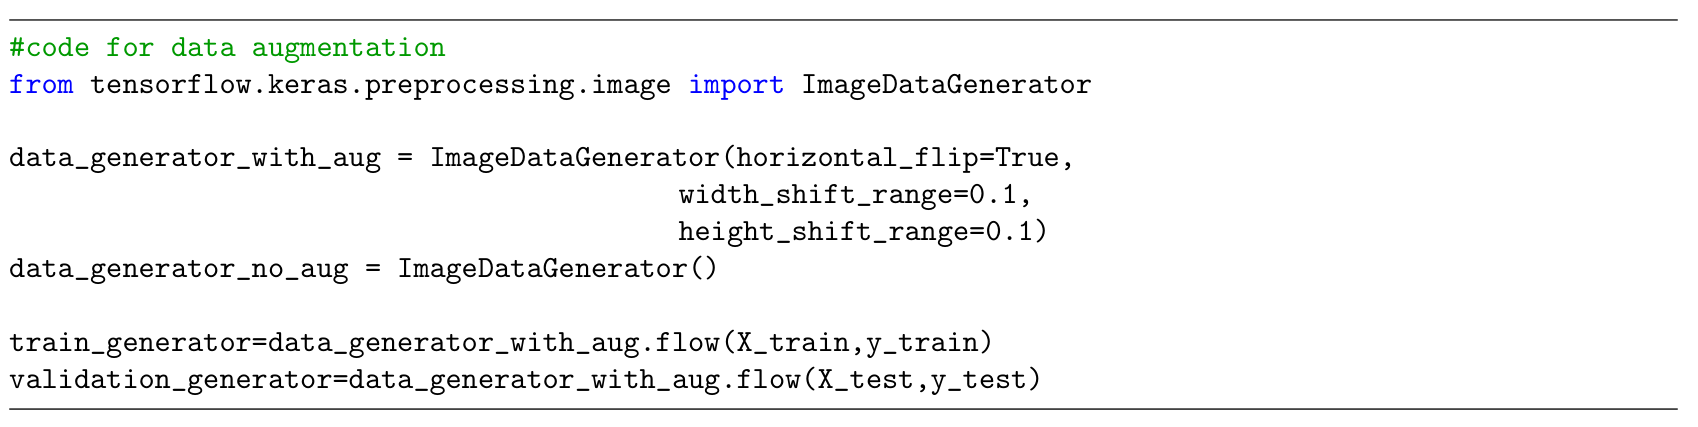
\includegraphics[scale=0.55]{code/fcode3.png}
\end{center}
% \begin{lstlisting}
% #code for data augmentation
% from tensorflow.keras.preprocessing.image import ImageDataGenerator

% data_generator_with_aug = ImageDataGenerator(horizontal_flip=True,
%                                               width_shift_range=0.1,
%                                               height_shift_range=0.1)
% data_generator_no_aug = ImageDataGenerator()

% train_generator=data_generator_with_aug.flow(X_train,y_train)
% validation_generator=data_generator_with_aug.flow(X_test,y_test)
% \end{lstlisting}

Data augmentation techniques were then used to enhance the dataset, such as horizontal flipping and random shifts, and these were applied using the ImageDataGenerator class from Keras.
Coming to the architecture of the model - A CNN model is defined using the Sequential class from Keras. \cite{keras}
\begin{center}
    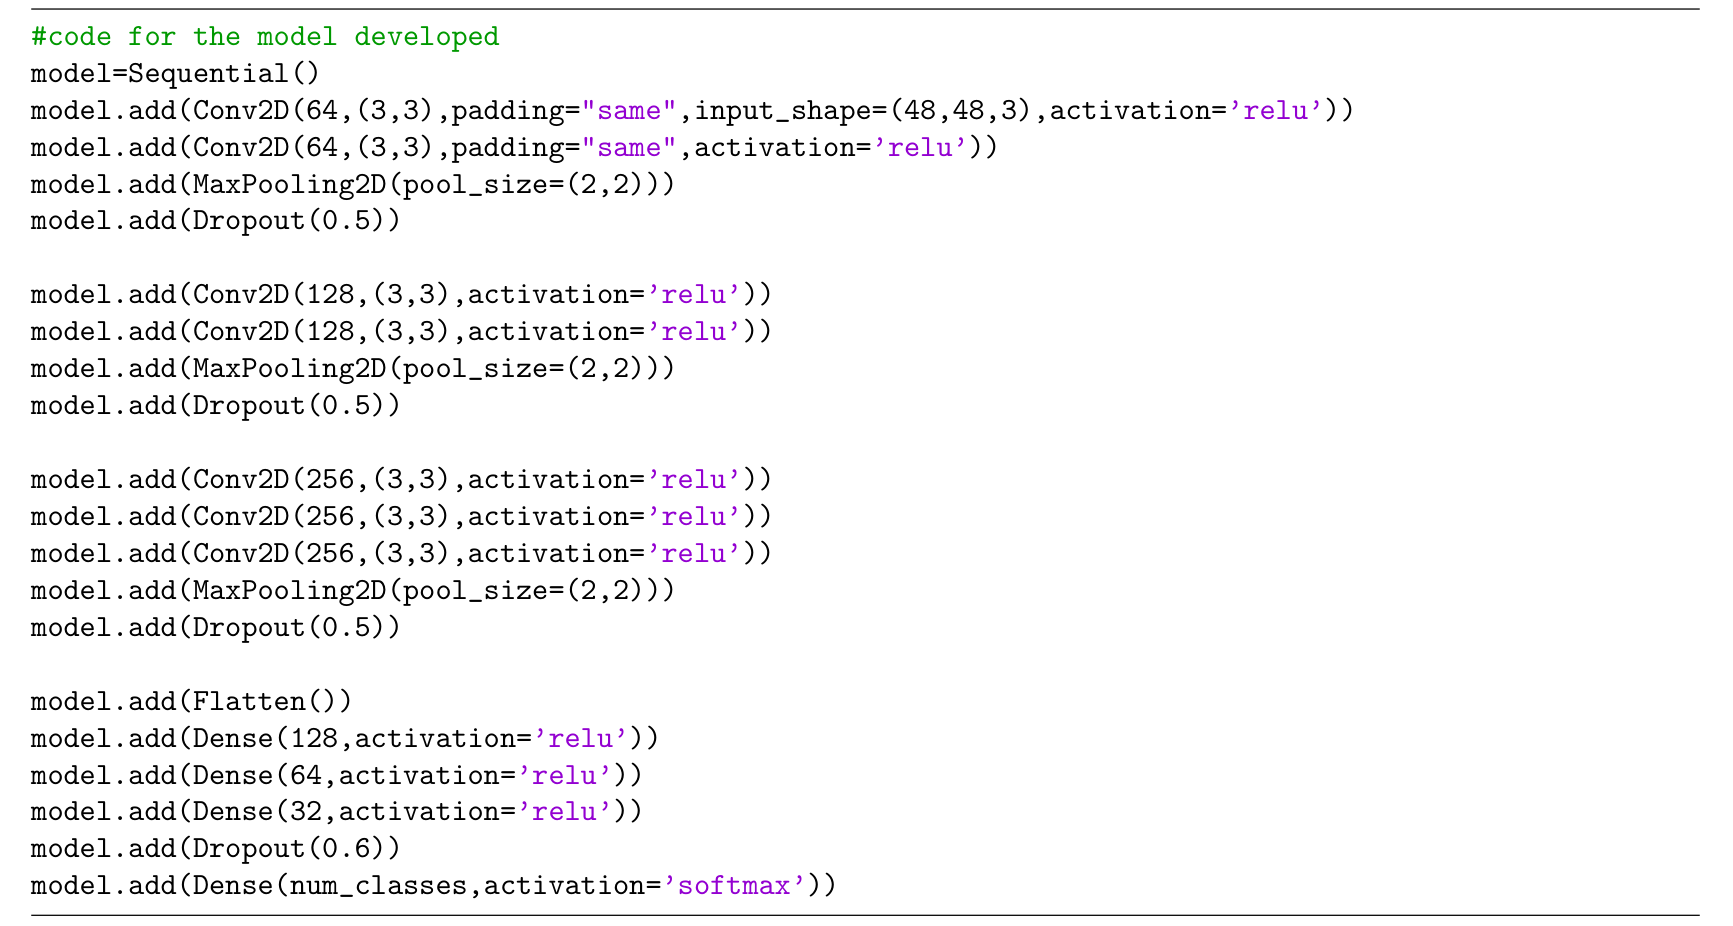
\includegraphics[scale=0.55]{code/fcode4.png}
 \end{center}
% \begin{lstlisting}
% #code for the model developed
% model=Sequential()
% model.add(Conv2D(64,(3,3),padding="same",input_shape=(48,48,3),activation='relu'))
% model.add(Conv2D(64,(3,3),padding="same",activation='relu'))
% model.add(MaxPooling2D(pool_size=(2,2)))
% model.add(Dropout(0.5))

% model.add(Conv2D(128,(3,3),activation='relu'))
% model.add(Conv2D(128,(3,3),activation='relu'))
% model.add(MaxPooling2D(pool_size=(2,2)))
% model.add(Dropout(0.5))

% model.add(Conv2D(256,(3,3),activation='relu'))
% model.add(Conv2D(256,(3,3),activation='relu'))
% model.add(Conv2D(256,(3,3),activation='relu'))
% model.add(MaxPooling2D(pool_size=(2,2)))
% model.add(Dropout(0.5))

% model.add(Flatten())
% model.add(Dense(128,activation='relu'))
% model.add(Dense(64,activation='relu'))
% model.add(Dense(32,activation='relu'))
% model.add(Dropout(0.6))
% model.add(Dense(num_classes,activation='softmax'))
% \end{lstlisting}
The model uses multiple convolutional layers, max-pooling layers, dropout layers, and dense layers to prevent overfitting. These layers are stacked together to create a deep neural network capable of learning meaningful representations from the input images.

The output of the last convolutional layer is flattened and passed through fully connected layers with progressively decreasing units. The final layer uses the softmax activation function to output the predicted probabilities for each class.

The training is performed using the `fit\_generator` method with the generated training and validation data. After training, the code visualizes the training and validation accuracy as well as the training and validation loss using Matplotlib.
The plot for the same is shown below:
\begin{figure}[H]
    \centering
    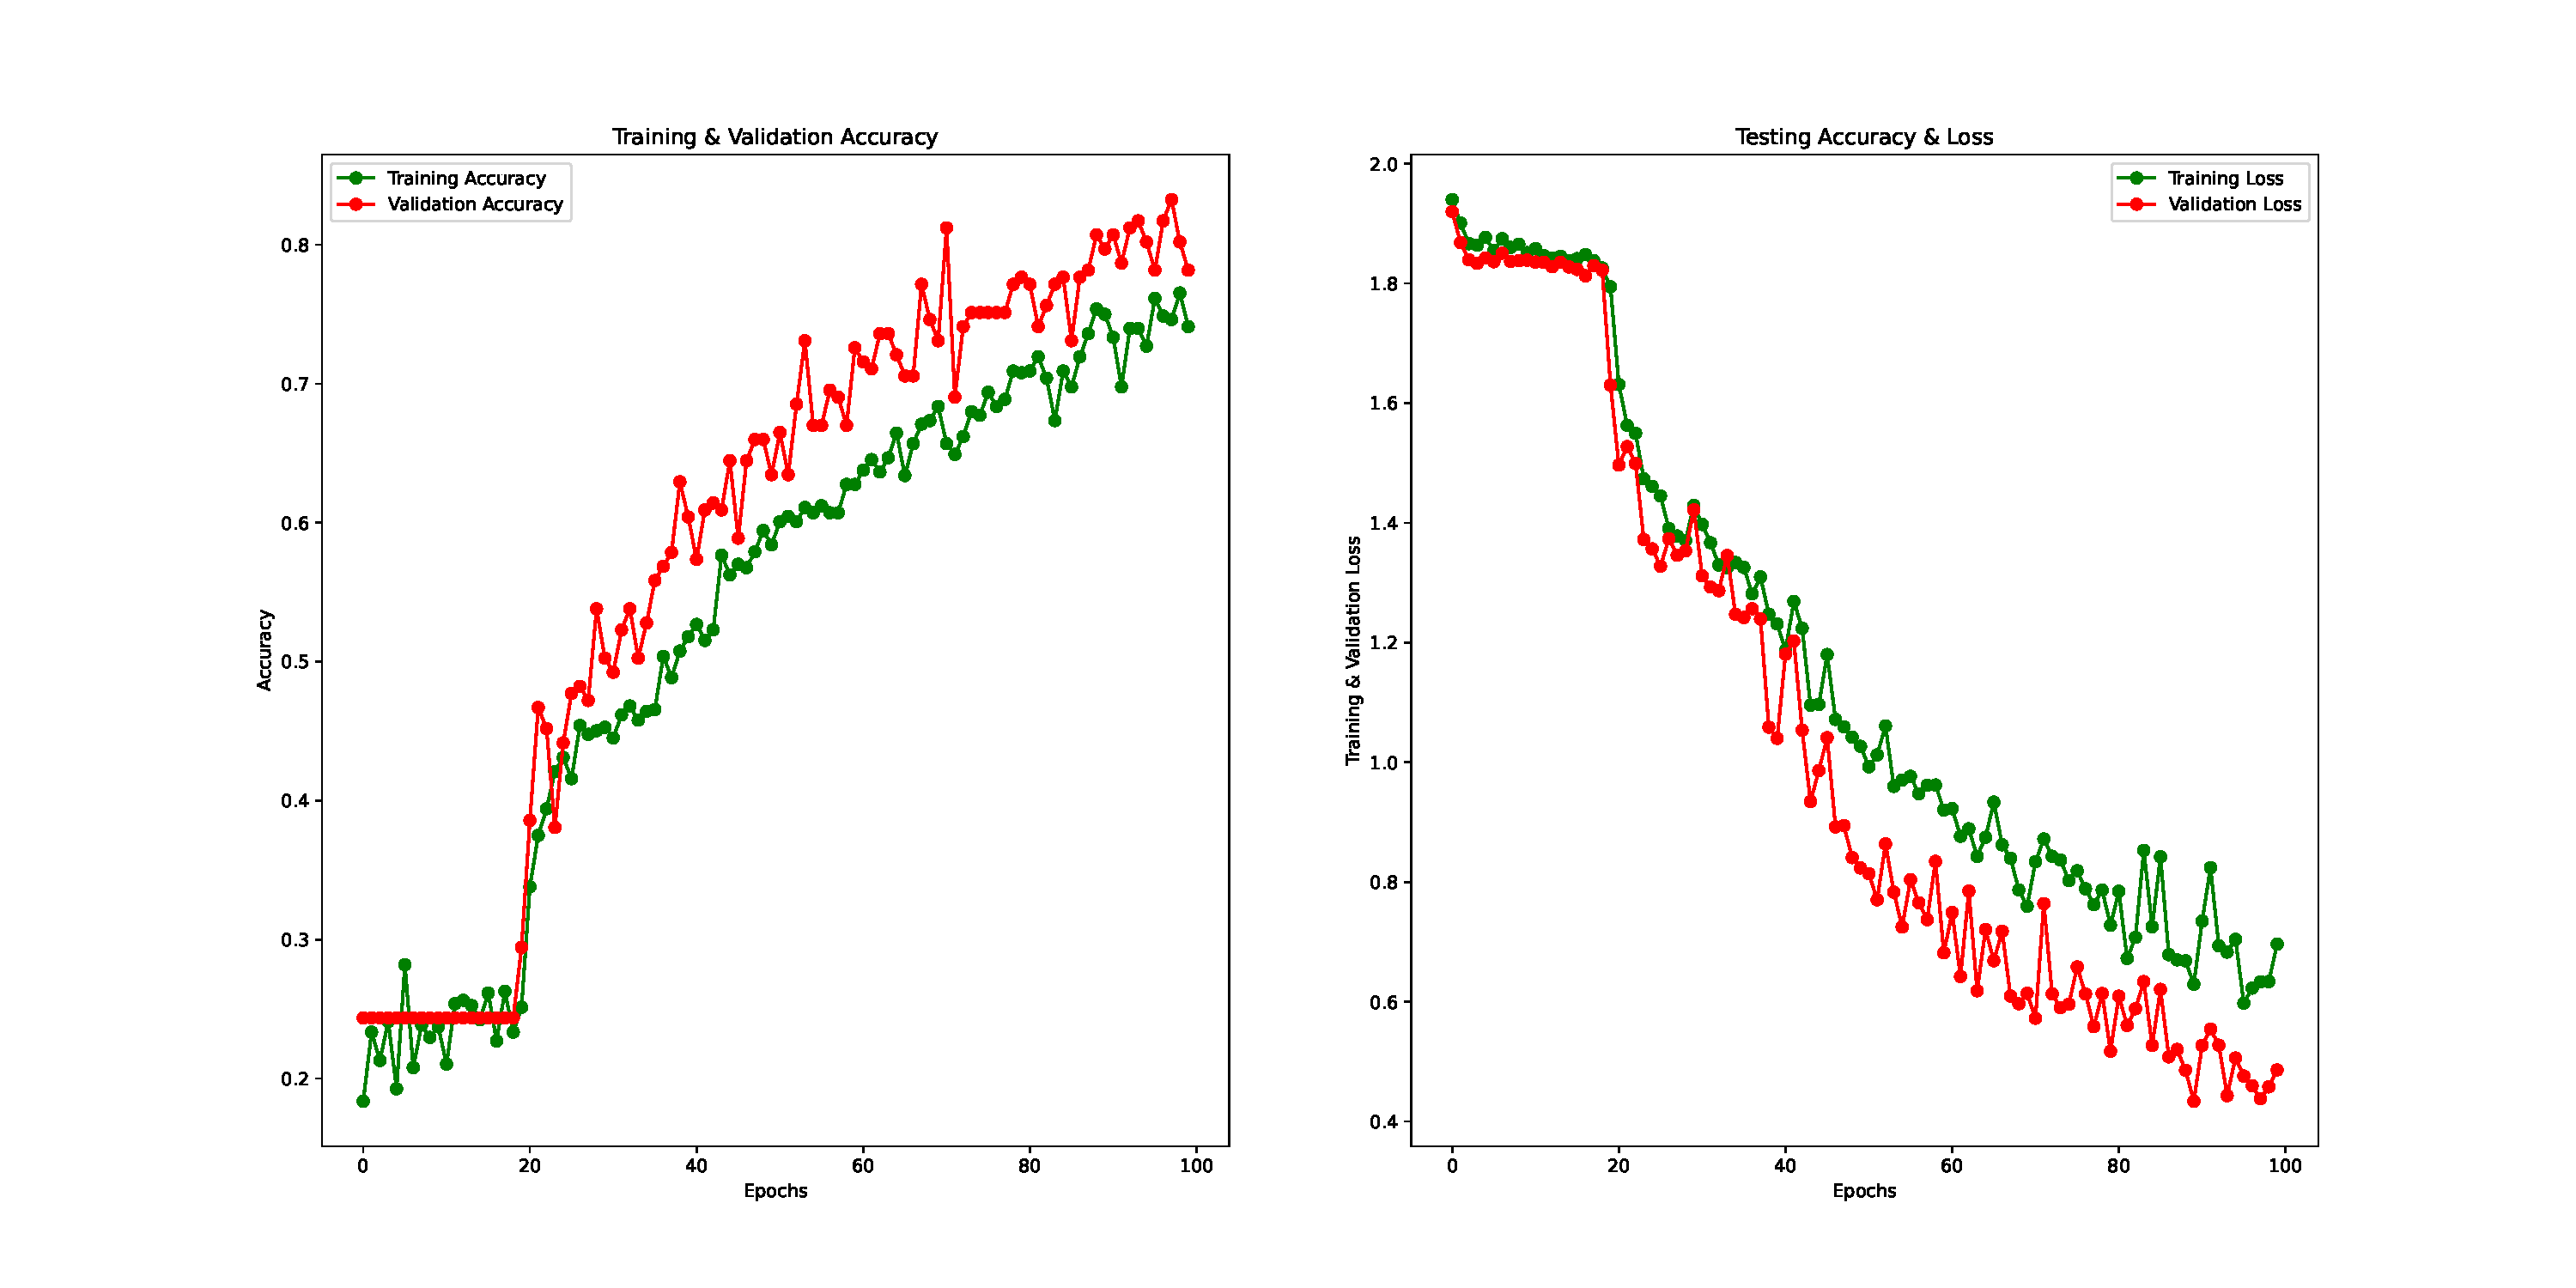
\includegraphics[scale= 0.4]{train-test.pdf}
    \caption{Accuracy and Loss}
    \label{fig:enter-label}
\end{figure}
We chose to use this model due to the following reasons - 
\begin{itemize}
    \item Max pooling layers, which are included in the model, aid in lowering spatial dimensions while keeping the most important properties. Additionally, dropout layers are used to minimise overfitting by arbitrarily deactivating certain neurons during training, improving generalisation.
    \item The model's capacity to adapt to changes in face expressions, positions, and lighting conditions is improved by the code's use of data augmentation techniques including horizontal flipping and random shifts. As a result, the model is stronger and better equipped to handle a variety of real-world events.
    \item In order to standardise the pixel values and improve the convergence and stability of the model during training, the image data is normalised by dividing it by 255.
    \item The dataset used to train the model contains a sizable number of facial photos depicting diverse moods. A more accurate and generalised model can be trained using a broad and extensive dataset.
    \item Accuracy and the confusion matrix are used to assess the model's performance. The confusion matrix sheds light on the model's capacity to distinguish between various emotion classes, while accuracy provides an overall measure of accurate predictions.
The programme produces visualisations of loss over epochs, training and validation accuracy, and both. These representations aid in evaluating the model's growth and spotting any problems like overfitting or underfitting.
Overall, the model is appropriate for facial recognition tasks because of the CNN architecture, data augmentation, normalisation, and assessment methodologies. It is useful for a variety of applications, including emotion analysis, affective computing, and human-computer interaction because of its potential to recognise and categorise face emotions with accuracy.

\end{itemize}
\section{Evaluation}

The code then evaluated the model's performance by predicting the classes for the test set and generating a confusion matrix using scikit-learn. 

The confusion matrix is displayed as a heatmap using Seaborn.The heatmap shows the distribution of predicted classes against the true classes, thus allowing us to asses the model’s performance in classifying different facial emotions. 

\begin{figure}[H]
    \centering
    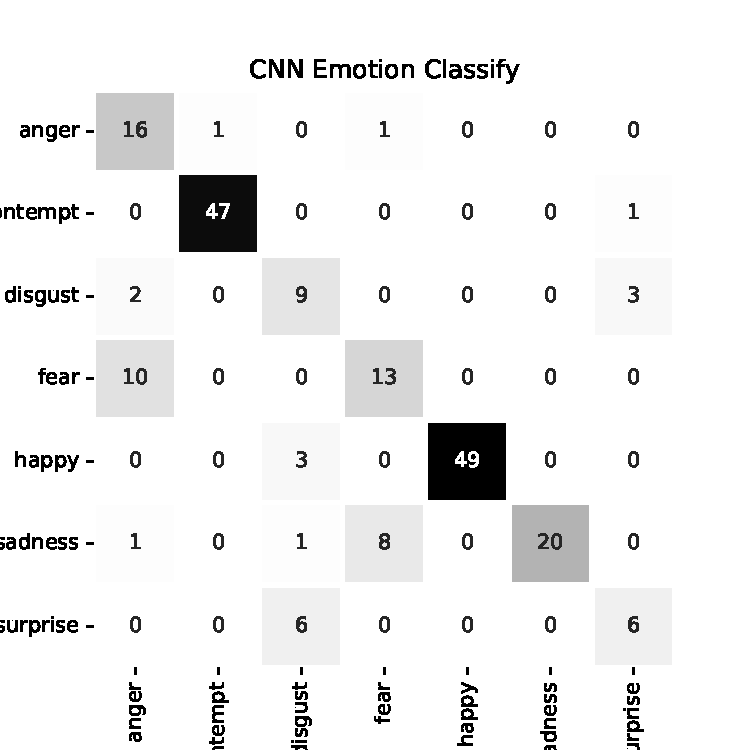
\includegraphics[scale=1]{confusion matrix.pdf}
    \caption{Confusion matrix}
    \label{fig:enter-label}
\end{figure}

\noindent Other than this it was observed that the model had an accuracy of 78.17\% which is higher than our threshold to reject the model which was 75\%.
\section{Deployment}
\subsection{Streamlit}
Streamlit is an open-source framework for creating web applications based in the
Python language. It is popularly used to create data science applications and
serves as a method to create a working prototype to test Machine Learning
models. Streamlit is favored by data scientists as it is compatible with major
Python libraries used for Deep Learning, such as scikit-learn, Keras, PyTorch,
SymPy(latex), NumPy, pandas, Matplotlib, etc. It enables data scientists to create
and share beautiful, custom web applications and does not require a thorough
knowledge of common web development languages and methods. Streamlit uses
React for its frontend to render the data on a screen and needs python version
>=3.7 to work.
The official Streamlit documentation has clearly laid out code snippets for
commonly used widgets like text elements, input widgets, layout widgets, media
elements, etc. We used the Streamlit library to create an application and deploy our Facial Expression Detection Model.

\subsection{Streamlit Code}
The web-based application for facial expression recognition is built using Streamlit and Tensorflow. \\ \\

\noindent The necessary libraries and the model are imported. The FacialExpressionModel is initialized with pre-trained weights. The model is designed to recognize seven different emotions: contempt, surprise, anger, disgust, fear, happiness, and sadness. The `choose\_image\_and\_predict` function handles image preprocessing and emotion prediction. It accepts an image, converts it to grayscale, resizes it to 48x48, and then makes a prediction using the previously initialized model. The application shows a demo image of the prediction. The users can upload an image, and the application will predict and display the emotion expressed in the image.
\\ \\
\noindent The following code was used -
\begin{center}
    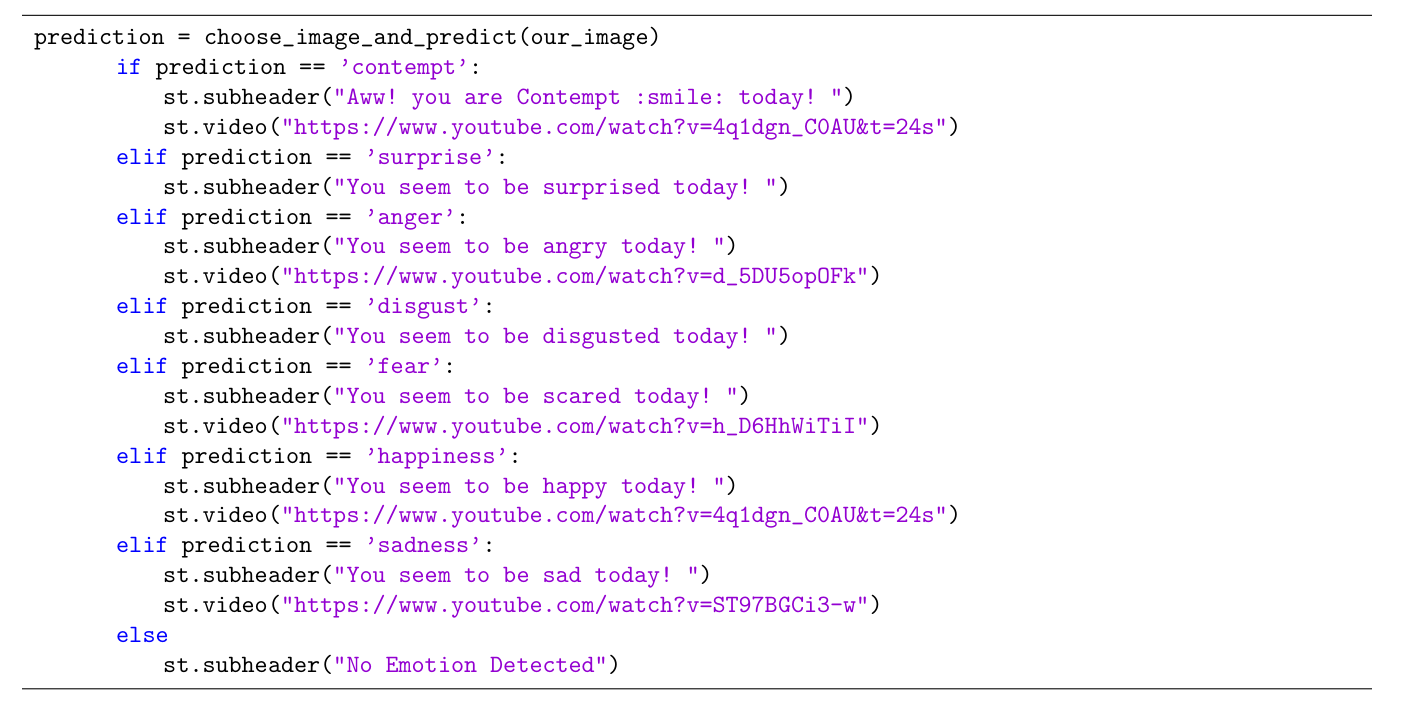
\includegraphics[scale=0.65]{code/fcode5.png}
\end{center}
% \begin{lstlisting}
%  prediction = choose_image_and_predict(our_image)
%         if prediction == 'contempt':
%             st.subheader("Aww! you are Contempt :smile: today! ")
%             st.video("https://www.youtube.com/watch?v=4q1dgn_C0AU&t=24s")
%         elif prediction == 'surprise':
%             st.subheader("You seem to be surprised today! ")
%         elif prediction == 'anger':
%             st.subheader("You seem to be angry today! ")
%             st.video("https://www.youtube.com/watch?v=d_5DU5opOFk")
%         elif prediction == 'disgust':
%             st.subheader("You seem to be disgusted today! ")
%         elif prediction == 'fear':
%             st.subheader("You seem to be scared today! ")
%             st.video("https://www.youtube.com/watch?v=h_D6HhWiTiI")
%         elif prediction == 'happiness':
%             st.subheader("You seem to be happy today! ")
%             st.video("https://www.youtube.com/watch?v=4q1dgn_C0AU&t=24s")
%         elif prediction == 'sadness':
%             st.subheader("You seem to be sad today! ")
%             st.video("https://www.youtube.com/watch?v=ST97BGCi3-w")
%         else 
%             st.subheader("No Emotion Detected")
% \end{lstlisting}

When an image is uploaded in the 'Detect your Facial expressions' section, it passes through the emotion prediction model. Depending on the predicted emotion, different responses, including text and videos, are shown to the user.

Streamlit code is easy to read and intuitive, which makes it the appropriate framework for coding basic data science applications. 
\pagebreak

\noindent Below are the screenshots from the web application built to exhibit the outcome of our trained model -  
\begin{center}
    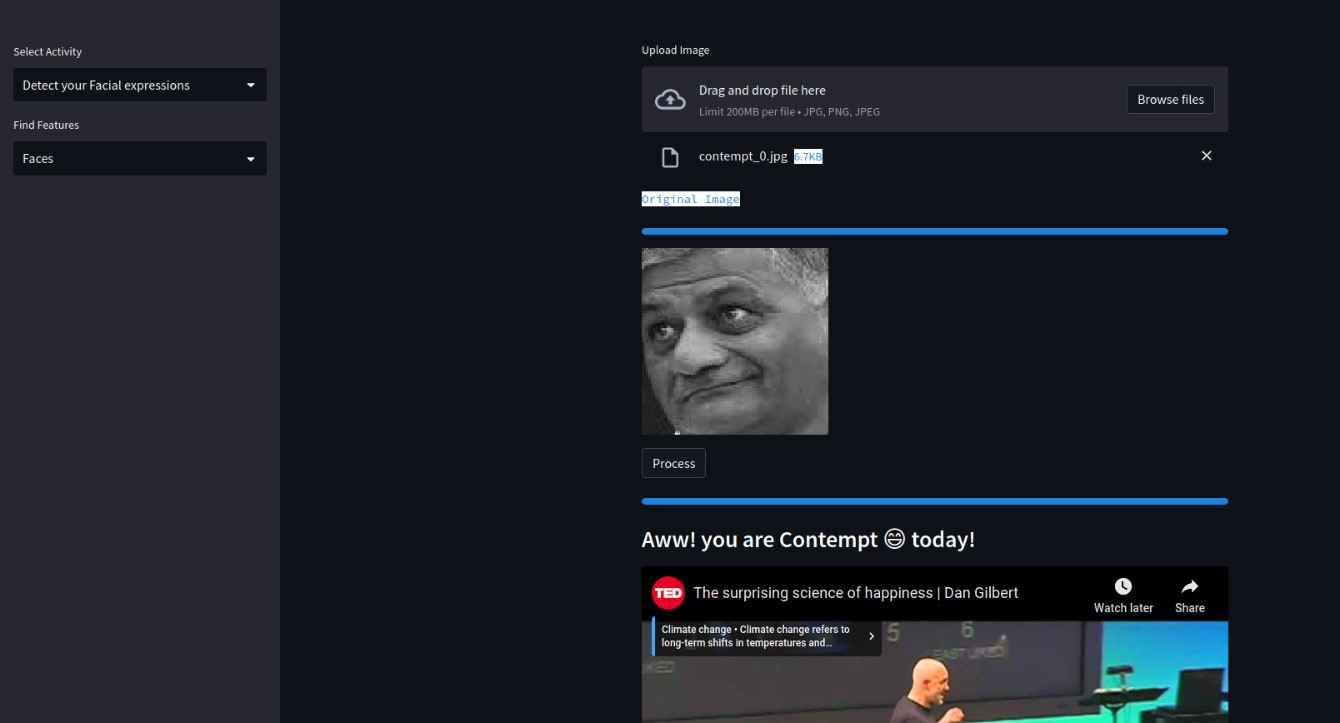
\includegraphics[scale=0.5]{streamlit images/image3.jpg}
\end{center}
\vspace{0.1in}
\begin{center}
    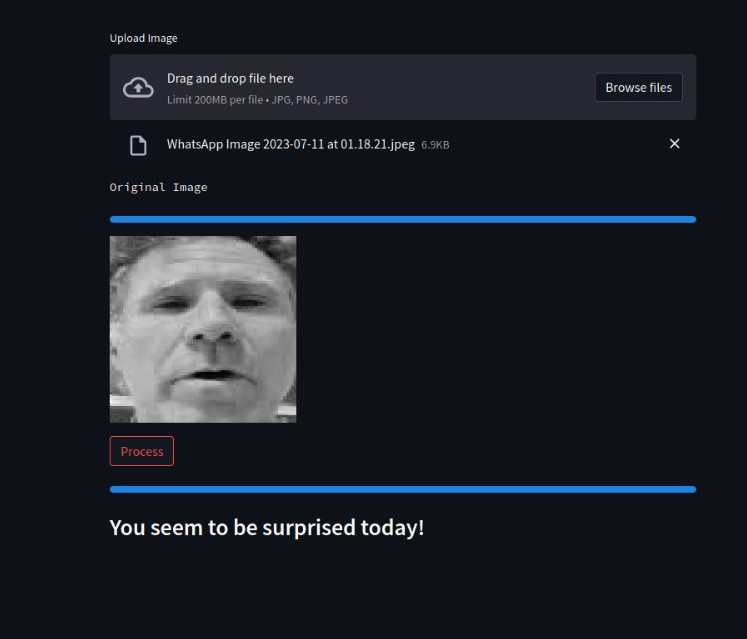
\includegraphics[scale=0.5]{streamlit images/image4.jpg}
    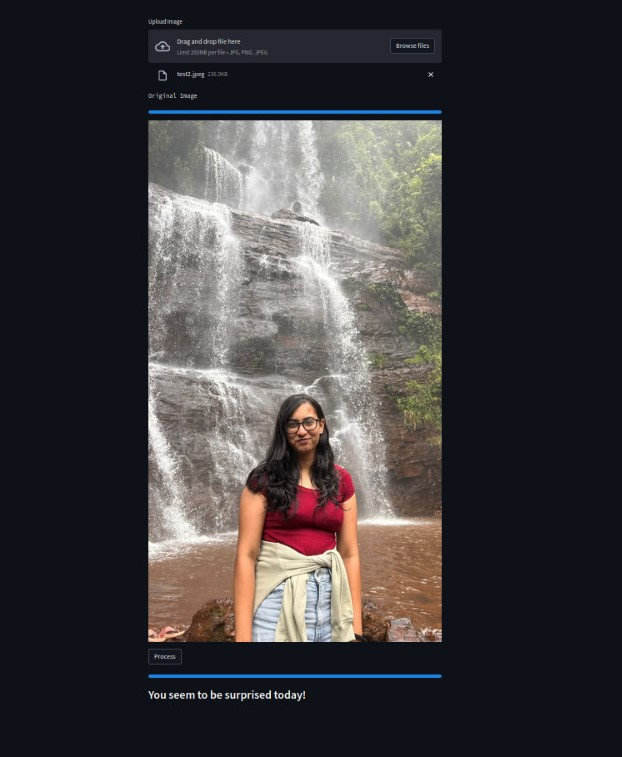
\includegraphics[scale=0.5]{streamlit images/image1.jpg}
\end{center}
\pagebreak
\section{Conclusion}
In summary, the facial emotion recognition model developed using CNN has distinguished itself with a commendable accuracy rate of 78.17\% in classifying seven distinct emotions: anger, contempt, fear, surprise, happiness, sadness, and disgust. This model can be used in various applications, such as psychology, marketing, and human-computer interaction.

There are many business and marketing implications when it comes to being able to correctly categorise a person's emotional state based on their facial expressions. Companies can determine areas where they need to improve their goods or services by looking for patterns in customer emotions. They can use this information to adjust their strategy appropriately, increasing client satisfaction and loyalty.

Additionally, people who find it difficult to express their emotions to a therapist fully can benefit from using the facial emotion recognition model in psychology. It can also compare emotions across cultures, helping researchers better understand how emotions are expressed in various societies.

The Streamlit library was used to deploy the model on a website, making it simple and approachable. The website is usable by various users because it can accept webcam and image upload input. This may make the facial emotion recognition model more widely applicable and have a more significant impact, allowing more people to gain from its applications and insights.

\section{Acknowledgements}
We are filled with immense gratitude to express our heartfelt appreciation to Dr. Aneesh Chivukula for providing us with the wonderful opportunity to work on designing this facial emotion recognition model. Throughout this journey, our team has learnt different technologies and dealt with uncertainty with a positive attitude. His astute insights and unwavering support have enabled us to design a facial emotion recognition model that is both accurate and efficient. With our teamwork, we learned many concepts of Deep Learning, Model Deployment and error handling in Machine Learning.  Once again, I express my deepest gratitude to Dr. Aneesh for this remarkable opportunity, which has enriched my knowledge and skills in the fascinating field of deep learning and image processing.

\addcontentsline{toc}{section}{References}
\printbibliography
\end{document}